\documentclass[10pt,a4paper]{article}
\usepackage{tocloft}
\usepackage{commons/course}
\usepackage{booktabs}
\usepackage{graphicx}
\usepackage{tikz}
\usetikzlibrary{arrows.meta,positioning,calc,decorations.pathreplacing,fit}

\definecolor{keywordstyle}{rgb}{0.0, 0.4, 0.8}
\definecolor{stringstyle}{rgb}{0.9, 0.17, 0.31}
\definecolor{commentstyle}{rgb}{0.1, 0.6, 0.2}
\definecolor{numberstyle}{rgb}{0.4, 0.4, 0.4}
\definecolor{backgroundcolor}{rgb}{0.94, 0.97, 1.0}

\lstdefinelanguage{ShellLike}{
	morekeywords={PASS,FAIL,Passed,Failed,Running,Loading,summary,iverilog},
	sensitive=false,
	morecomment=[l]{\#},
	morestring=[b]",
}

\lstset{
	language=ShellLike,
	basicstyle=\ttfamily\scriptsize,
	keywordstyle=\color{keywordstyle}\bfseries,
	stringstyle=\color{stringstyle},
	commentstyle=\color{commentstyle},
	numbers=none,
	keepspaces=true,
	tabsize=2,
	showspaces=false,
	showstringspaces=false,
	showtabs=false,
	breaklines=true,
	breakatwhitespace=false,
	frame=single,
	backgroundcolor=\color{backgroundcolor},
}

\lstdefinestyle{verilog}{
	language=Verilog,
	basicstyle=\ttfamily\scriptsize,
	keywordstyle=\color{keywordstyle}\bfseries,
	commentstyle=\color{commentstyle},
	stringstyle=\color{stringstyle},
	numbers=left,
	numberstyle=\tiny\color{numberstyle},
	frame=single,
	backgroundcolor=\color{backgroundcolor},
	breaklines=true,
	tabsize=2,
}

\newlistof{listofproblems}{lop}{\normalsize فهرست مسائل}
\newcommand{\addproblem}[1]{\addcontentsline{lop}{listofproblems}{\protect\numberline{}#1}}


\begin{document}

\سربرگ{آزمایش نهم}{پیاده‌سازی حافظه‌ی شرکت‌پذیر سه‌گانه (\lr{TCAM})}{}{استاد: دکتر انصاری}

\subsubsection*{خلاصه}

در این آزمایش یک پیمانه‌ی \lr{TCAM} به اندازه‌ی ۱۶ ثبات ۱۶ بیتی طراحی و پیاده‌سازی شده است.

حافظه‌ی معمولی با {آدرس} کار می‌کند: آدرس می‌دهی و محتوا می‌گیری. حافظه‌ی شرکت‌پذیر (\lr{CAM}) برعکس عمل می‌کند: {محتوا} می‌دهی و آدرس می‌گیری، و این کار را با مقایسه‌ی هم‌زمان همه‌ی خانه‌ها انجام می‌دهد. \lr{TCAM} یک قدم جلوتر می‌رود و اجازه می‌دهد در هر خانه، علاوه بر $0$ و $1$، نماد سوم $X$ هم ذخیره شود که یعنی «این جایگاه مقایسه نشود».

\subsubsection*{نماد سوم چطور ذخیره می‌شود}

سخت‌افزار سطح منطقی سومی برای ذخیره کردن ندارد، پس هر بیت با {دو} فلیپ‌فلاپ نگه داشته می‌شود:

\begin{center}
\begin{tabular}{@{}lll@{}}
\toprule
\lr{care} & \lr{value} & {نماد ذخیره‌شده} \\
\midrule
$1$ & $0$ & $0$ \\
$1$ & $1$ & $1$ \\
$0$ & --- & $X$ (مقدار بی‌اهمیت است) \\
\bottomrule
\end{tabular}
\end{center}

و یک جایگاه وقتی با بیت جست‌وجو {موافق} است که:

\[
\text{agree} \;=\; \overline{\text{care}} \;+\; \overline{(\text{value} \oplus \text{search})}
\]

یعنی یا اصلا قرار نیست مقایسه شود، یا مقایسه شده و برابر درآمده است. کل سلول سه‌گانه همین است:

\begin{latin}
\lstinputlisting[style=verilog]{../rtl/tcam_cell.v}
\end{latin}

\subsubsection*{چرا بیت اعتبار اختیاری نیست}

نکته‌ای که در نگاه اول دیده نمی‌شود ولی مدار را از کار می‌اندازد این است: خانه‌ای که همه‌ی بیت‌های \lr{care} آن صفر باشد، کاملا $X$ است و {با هر کلمه‌ای منطبق می‌شود}.

پس از ریست، فلیپ‌فلاپ‌های \lr{care} صفرند. بنابراین یک \lr{TCAM} خالی — بدون بیت اعتبار — برای {هر} ورودی، شانزده انطباق گزارش می‌کرد. بیت اعتبار در هر خانه دقیقا جلوی همین را می‌گیرد و به‌عنوان یک ورودی جداگانه‌ی نوشتن هم بیرون داده شده است، تا بشود یک قاعده را {بازنشسته} کرد بدون اینکه محتوایش پاک شود.

\begin{center}
\lr{match$_i$ = valid$_i$ $\wedge$ ($\bigwedge_k$ agree$_{i,k}$)}
\end{center}

این ویژگی در تست‌بنچ صریحا بررسی شده است: هم اینکه \lr{TCAM} خالی هرگز انطباق نمی‌دهد، و هم اینکه خانه‌ی تماما $X$ پس از معتبر شدن با هر کلمه‌ای منطبق می‌شود.

\begin{latin}
\lstinputlisting[style=verilog]{../rtl/tcam_entry.v}
\end{latin}

\subsubsection*{مثال صورت آزمایش}

صورت آزمایش می‌گوید اگر داده‌ی \lr{01101110} در \lr{TCAM} جست‌وجو شود، هر سه الگوی زیر انطباق دارند. رمزگذاری مقدار و ماسک هر کدام به این شکل درمی‌آید:

\begin{center}
\begin{tabular}{@{}llll@{}}
\toprule
{الگو} & \lr{care} & \lr{value} & {نتیجه برای \lr{01101110}} \\
\midrule
\lr{X1101XXX} & \lr{01111000} & \lr{01101000} & انطباق \\
\lr{0X1X11X0} & \lr{10101101} & \lr{00101100} & انطباق \\
\lr{0110XXXX} & \lr{11110000} & \lr{01100000} & انطباق \\
\midrule
\lr{1XXXXXXX} & \lr{10000000} & \lr{10000000} & بدون انطباق \\
\lr{01101111} & \lr{11111111} & \lr{01101111} & بدون انطباق \\
\bottomrule
\end{tabular}
\end{center}

بررسی سطر اول به‌صورت دستی: \lr{01101110 $\oplus$ 01101000 = 00000110} و \lr{00000110 $\wedge$ 01111000 = 00000000}، پس هیچ جایگاهی که قرار بوده مقایسه شود مخالفت نکرده است.

الگوهای صورت آزمایش ۸ بیتی‌اند و این \lr{TCAM} ۱۶ بیتی است، پس بایت بالای هر الگو تماما $X$ گذاشته شده است. این یک دور زدن مسئله نیست؛ روش عادی ذخیره‌ی یک قاعده‌ی باریک در یک \lr{TCAM} پهن‌تر همین است، و در تست‌بنچ با جست‌وجوی همان داده با {دو بایت بالای متفاوت} بررسی شده است.

\subsubsection*{چند انطباق هم‌زمان و اولویت}

در مثال بالا یک کلمه‌ی جست‌وجو با سه قاعده منطبق شد. این حالت عادی است نه خطا — کل فایده‌ی \lr{TCAM} همین است که قاعده‌های هم‌پوشان ذخیره شوند. اما چیزی باید انتخاب کند، و قرارداد تقریبا همه‌جایی این است که {آدرس کوچک‌تر برنده است}، تا قاعده‌های خاص‌تر جلوتر نوشته شوند.

\begin{latin}
\lstinputlisting[style=verilog]{../rtl/priority_encoder.v}
\end{latin}

علاوه بر آدرس برنده، {تعداد} خانه‌های منطبق هم بیرون داده می‌شود. این خروجی تزئینی نیست: تفاوت میان «یک قاعده این کلمه را پوشش می‌دهد» و «چهار قاعده آن را پوشش می‌دهند» اطلاعات واقعی است، و از نظر تست تنها راهی است که می‌شود کدگذار اولویت درست را از کدگذاری که {اتفاقی} خانه‌ی درست را انتخاب کرده تشخیص داد.

\subsubsection*{پیمانه‌ی کامل}

\begin{center}
\begin{latin}
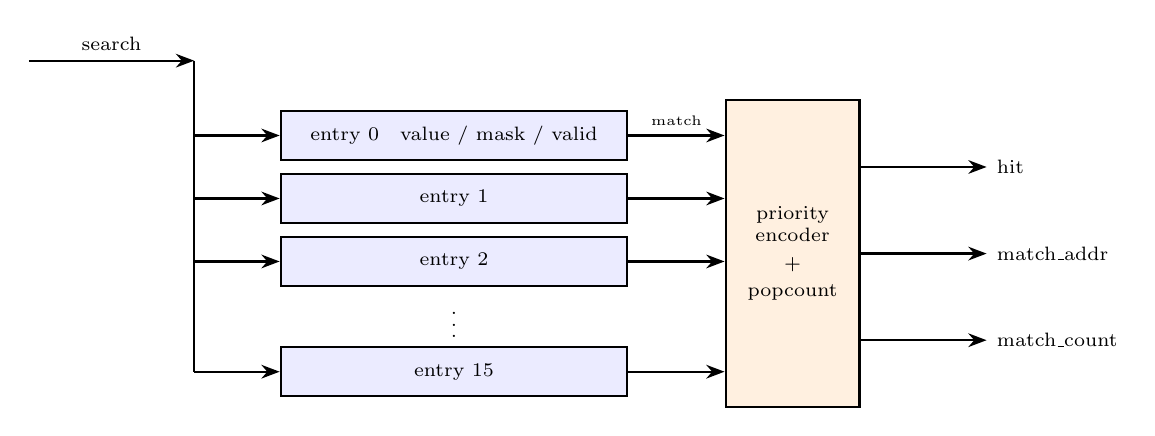
\begin{tikzpicture}[
  ent/.style={draw, minimum height=0.62cm, minimum width=4.4cm, align=center,
              font=\scriptsize, inner sep=1pt},
  >=Stealth, thick
]
  \node[ent, fill=blue!8]  (e0)  at (0,0)     {entry 0 \; value / mask / valid};
  \node[ent, fill=blue!8]  (e1)  at (0,-0.8)  {entry 1};
  \node[ent, fill=blue!8]  (e2)  at (0,-1.6)  {entry 2};
  \node[font=\scriptsize]        at (0,-2.3)  {$\vdots$};
  \node[ent, fill=blue!8]  (e15) at (0,-3.0)  {entry 15};

  \node[draw, minimum width=1.7cm, minimum height=3.9cm, align=center,
        font=\scriptsize, fill=orange!12] (pri) at (4.3,-1.5)
        {priority\\encoder\\[2pt]+\\[2pt]popcount};

  % search word broadcast to every entry
  \draw[thick] (-3.3,0.95) -- (-3.3,-3.0);
  \draw[->] (-5.4,0.95) -- (-3.3,0.95)
      node[midway, above, font=\scriptsize]{search};
  \draw[->] (-3.3,-0.8)  -- (e1.west);
  \draw[->] (-3.3,-1.6)  -- (e2.west);
  \draw[->] (-3.3,-3.0)  -- (e15.west);
  \draw[->] (-3.3,0)     -- (e0.west);

  % match lines
  \draw[->] (e0.east)  -- (e0.east  -| pri.west) node[midway,above,font=\tiny]{match};
  \draw[->] (e1.east)  -- (e1.east  -| pri.west);
  \draw[->] (e2.east)  -- (e2.east  -| pri.west);
  \draw[->] (e15.east) -- (e15.east -| pri.west);

  \draw[->] ($(pri.east)+(0,1.1)$)  -- ++(1.6,0) node[right,font=\scriptsize]{hit};
  \draw[->] ($(pri.east)+(0,0)$)    -- ++(1.6,0) node[right,font=\scriptsize]{match\_addr};
  \draw[->] ($(pri.east)+(0,-1.1)$) -- ++(1.6,0) node[right,font=\scriptsize]{match\_count};
\end{tikzpicture}
\end{latin}
\end{center}

کلمه‌ی جست‌وجو به {همه‌ی} خانه‌ها هم‌زمان پخش می‌شود و مسیر از ورودی تا خطوط انطباق کاملا {ترکیبی} است. حافظه فقط در محتواست، نه در جست‌وجو؛ و همین است که یک \lr{CAM} را \lr{CAM} می‌کند: یک جست‌وجو به اندازه‌ی یک زنجیره‌ی تاخیر گیت طول می‌کشد، نه شانزده خواندن از حافظه.

در پیاده‌سازی روی \lr{FPGA} معمولا خروجی‌ها را ثبات‌دار می‌کنند تا بستن زمان‌بندی ساده شود. اینجا این کار عمدا انجام نشده تا پیمانه دقیقا همان جست‌وجوی شرکت‌پذیری باشد که صورت آزمایش توصیف کرده، بدون هیچ چیز اضافه‌ای در مسیر.

\begin{latin}
\lstinputlisting[style=verilog]{../rtl/tcam.v}
\end{latin}

\subsubsection*{شکل موج}

\begin{center}
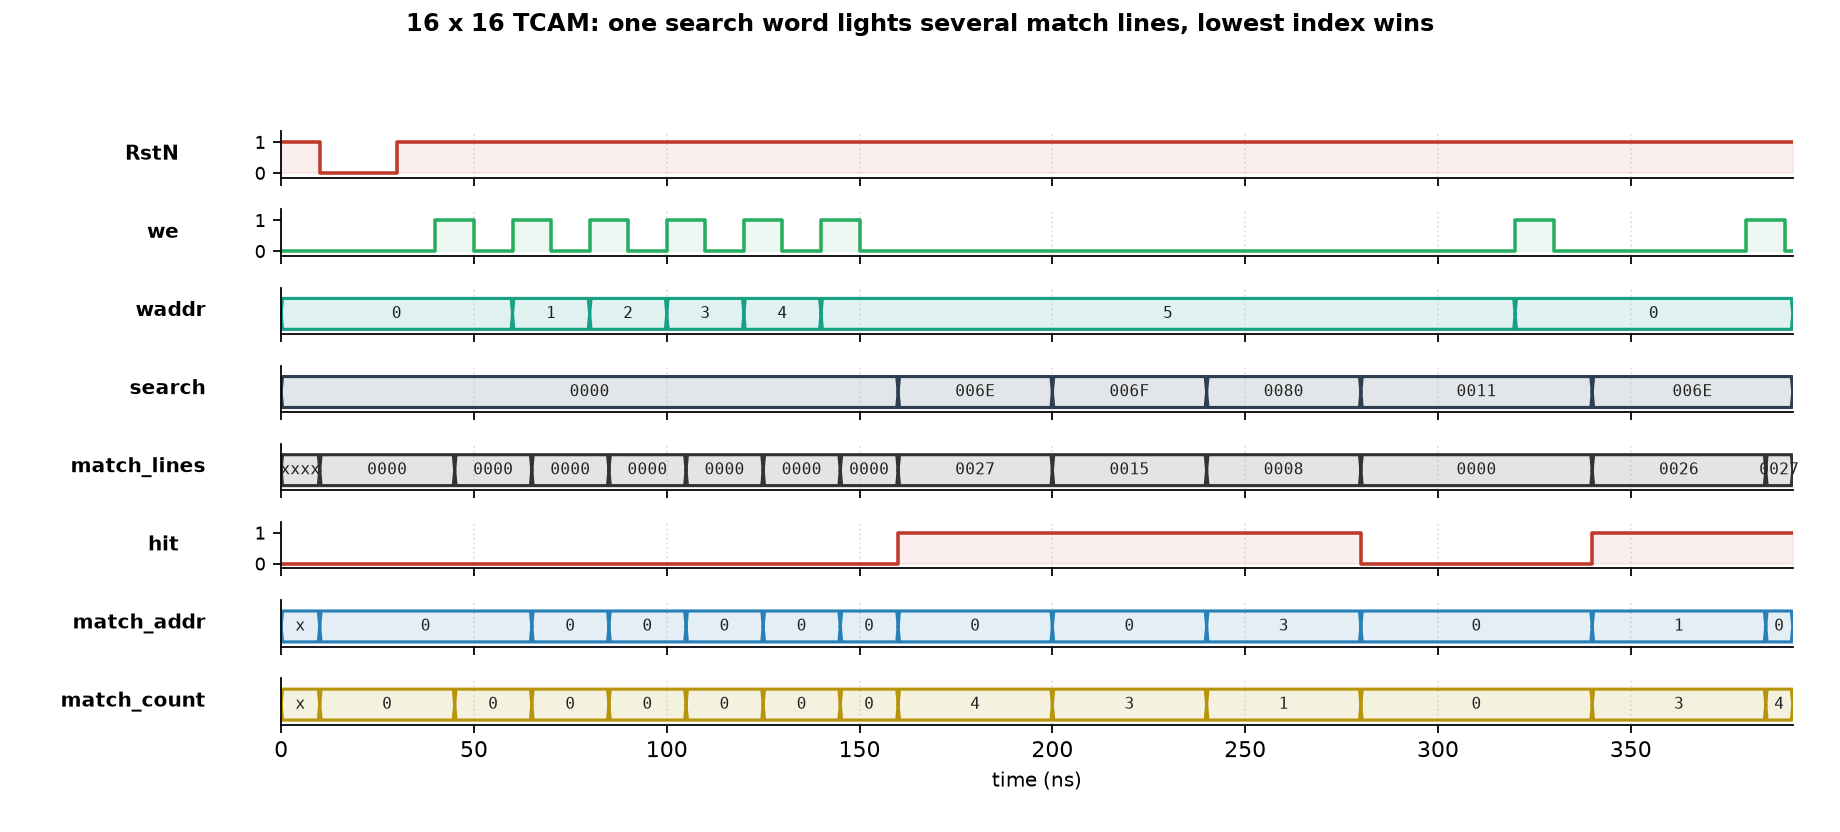
\includegraphics[width=\textwidth]{figs/wave_tcam.png}\\[0.4em]
\end{center}

شش الگوی جدول بالا در خانه‌های $0$ تا $5$ نوشته شده‌اند و سپس چند کلمه جست‌وجو می‌شود:

\begin{center}
\begin{tabular}{@{}lllll@{}}
\toprule
{جست‌وجو} & \lr{match\_lines} & {خانه‌های منطبق} & \lr{count} & \lr{addr} \\
\midrule
\lr{0x006E} & \lr{0x0027} & $0,1,2,5$ & $4$ & $0$ \\
\lr{0x006F} & \lr{0x0015} & $0,2,4$   & $3$ & $0$ \\
\lr{0x0080} & \lr{0x0008} & $3$       & $1$ & $3$ \\
\lr{0x0011} & \lr{0x0000} & ---       & $0$ & --- \\
\midrule
\multicolumn{5}{@{}l@{}}{\small پس از بازنشسته کردن خانه‌ی $0$:} \\
\lr{0x006E} & \lr{0x0026} & $1,2,5$   & $3$ & $1$ \\
\bottomrule
\end{tabular}
\end{center}

سطر اول همان مثال صورت آزمایش است. سطر دوم جالب‌تر است: \lr{01101111} فقط در آخرین بیت با داده‌ی قبلی فرق دارد، ولی مجموعه‌ی قاعده‌های منطبق کاملا عوض می‌شود — \lr{0X1X11X0} آن را رد می‌کند چون آخرین بیتش باید صفر باشد، و در عوض قاعده‌ی دقیق \lr{01101111} حالا منطبق است.

دو سطر آخر رفتار اولویت را نشان می‌دهد: به‌محض بازنشسته شدن خانه‌ی $0$، خانه‌ی $1$ برنده می‌شود و شمارنده یکی کم می‌شود، بدون اینکه محتوای خانه‌ی $0$ پاک شده باشد.

توجه کنید که وقتی \lr{hit} پایین است، مقدار \lr{match\_addr} بی‌معنی است. کدگذار اولویت در نبود هیچ انطباقی صفر بیرون می‌دهد و صفر یک آدرس معتبر است، پس مصرف‌کننده {باید} اول \lr{hit} را ببیند. همین نکته باعث شد در تست‌بنچ، بررسی آدرس فقط زمانی انجام شود که مدل مرجع انتظار انطباق داشته باشد.

\subsubsection*{تست‌ها}

چهار تست‌بنچ نوشته شده که از پایین به بالا مدار را می‌پوشانند.

\textbf{۱) سلول سه‌گانه — کامل.} یک سلول فقط سه ورودی مؤثر دارد (مقدار ذخیره‌شده، بیت \lr{care} و بیت جست‌وجو)، پس «کامل» اینجا واقعا یعنی هر هشت ترکیب، در برابر جدول درستی‌ای که مستقیم از تعریف سه نماد $\{0,1,X\}$ نوشته شده است.

\begin{latin}
\lstinputlisting[style=verilog]{../tb/tb_tcam_cell.v}
\end{latin}

\textbf{۲) یک خانه — جاروب کامل فضای جست‌وجو.} یک خانه‌ی ۱۶ بیتی فقط $65536$ کلمه‌ی جست‌وجوی ممکن دارد، پس برای هر الگوی ذخیره‌شده می‌شود {همه‌ی} آن‌ها را بررسی کرد؛ نه نمونه‌برداری و نه زیرمجموعه‌ی تصادفی.

علاوه بر خود خط انطباق، {تعداد} کلمه‌های منطبق هم شمرده و با مقدار نظری مقایسه می‌شود. الگویی با $n$ بیت $X$ باید دقیقا با $2^n$ کلمه منطبق شود:

\begin{center}
\begin{tabular}{@{}lll@{}}
\toprule
{الگو} & {بیت‌های $X$} & {تعداد کلمه‌های منطبق} \\
\midrule
\lr{mask = 0xFFFF} & $0$  & $1$ \\
\lr{mask = 0xFF00} & $8$  & $256$ \\
\lr{mask = 0x0F0F} & $8$  & $256$ \\
\lr{mask = 0x8001} & $14$ & $16384$ \\
\lr{mask = 0x0000} & $16$ & $65536$ \\
\bottomrule
\end{tabular}
\end{center}

این بررسی چیزی می‌گیرد که مقایسه‌ی تک‌تک نمی‌گیرد: اگر یک بیت \lr{care} به سلول اشتباهی وصل شده باشد، برای بیشتر کلمه‌ها پاسخ همچنان درست درمی‌آید ولی {اندازه} مجموعه‌ی منطبق عوض می‌شود.

\begin{latin}
\lstinputlisting[style=verilog]{../tb/tb_tcam_entry.v}
\end{latin}

\textbf{۳) پیمانه‌ی کامل در برابر مدل مرجع.} مدل چند خط رفتاری بدون سلول، بدون کدگذار اولویت و بدون درخت شمارش است، پس نمی‌تواند اشتباه ساختاری طراحی را تکرار کند.

مهم‌تر از خود مدل، {نحوه‌ی راندن} آن است: هم محتوای \lr{TCAM} و هم کلمه‌های جست‌وجو تصادفی‌اند، و ماسک‌ها عمدا به سمت داشتن $X$ زیاد سوگیری شده‌اند (\lr{\$random \& \$random}). دلیلش این است که رفتار جالب \lr{TCAM} وقتی ظاهر می‌شود که قاعده‌ها {هم‌پوشانی} داشته باشند، و مجموعه‌ی بردارهای دست‌نویس دقیقا از هم‌پوشانی پرهیز می‌کند. در پایان، یک پیکربندی هم روی تمام $65536$ کلمه‌ی ممکن جاروب می‌شود تا دست‌کم یک نقشه‌ی کامل از فضای انطباق بررسی شده باشد، نه نمونه‌برداری‌شده.

\begin{latin}
\lstinputlisting[style=verilog]{../tb/tb_tcam.v}
\end{latin}

\textbf{۴) انطباق مستقیم با صورت آزمایش.} در این تست‌بنچ الگوها به‌صورت {متن} و با همان نماد $\{0,1,X\}$ صورت آزمایش نوشته می‌شوند و خود تست‌بنچ آن‌ها را به زوج مقدار/ماسک تبدیل می‌کند:

\begin{latin}
\begin{lstlisting}[style=verilog,numbers=none]
store_pattern(4'd0, "XXXXXXXXX1101XXX");
store_pattern(4'd1, "XXXXXXXX0X1X11X0");
store_pattern(4'd2, "XXXXXXXX0110XXXX");
\end{lstlisting}
\end{latin}

این کار دو فایده دارد. اول اینکه بررسی‌ها کنار صورت آزمایش خوانا می‌مانند. دوم و مهم‌تر اینکه {خود رمزگذاری مقدار/ماسک} بخشی از چیزی می‌شود که آزموده می‌شود: اگر رمزگذاری غلط بود، مثال کار شده‌ی صورت آزمایش از انطباق می‌افتاد.

\begin{latin}
\lstinputlisting[style=verilog]{../tb/tb_tcam_spec.v}
\end{latin}

\subsubsection*{نتایج تست}

\begin{latin}
\lstinputlisting[basicstyle=\ttfamily\scriptsize]{figs/test_run_output.txt}
\end{latin}

\subsubsection*{جمع‌بندی}

\lr{TCAM} از نظر منطقی ساده است — دو فلیپ‌فلاپ و سه گیت به ازای هر بیت — ولی دو نکته‌ی طراحی دارد که هیچ‌کدام از خود فرمول مقایسه بیرون نمی‌آید.

اول، بیت اعتبار. چون نماد $X$ با {نبود} \lr{care} کدگذاری می‌شود، حالت خالی مدار به‌طور طبیعی «با همه‌چیز منطبق شو» است نه «با هیچ‌چیز منطبق نشو». یعنی امن‌ترین حالت پس از ریست، بدترین حالت رفتاری است، و بیت اعتبار تنها چیزی است که آن را برمی‌گرداند.

دوم، اولویت. برخلاف حافظه‌ی معمولی که هر آدرس یک پاسخ دارد، پاسخ \lr{TCAM} می‌تواند چندتایی باشد. این ابهام ذاتی مسئله است، نه اشکال پیاده‌سازی، و باید با یک قرارداد صریح — اینجا «آدرس کوچک‌تر برنده است» — حل شود. خروجی \lr{match\_count} برای همین اضافه شد: بدون آن، تست‌بنچ نمی‌توانست تشخیص دهد که کدگذار اولویت درست کار می‌کند یا فقط اتفاقی خانه‌ی درست را برگردانده است.

\end{document}
